
\section{System Overview} Havven is designed to incentivise stability in a decentralised cryptocurrency denominated in some external currency, such as the USD. The dual-token asset system is combined with a set of novel incentive mechanisms designed to stabilise the price of one of the two tokens. We refer to these as the Havven token (\HAV{}) - to avoid confusion with the system itself - and the nomin, \NOM{} (short for denominator). \\

\noindent \HAV{} serves two functions:

\begin{enumerate}
\item{To provide the system with collateral (the system itself it tokenised), and,}
\item{To allow actors to contribute to the price stabilisation process through a set of incentives.}
\end{enumerate}

\noindent The second token, \NOM{}, is the stablecoin. The purpose of \NOM{} is to track the price of a chosen external denominating currency via the actions of \HAV{} token holders; holders of \HAV{} participate in modifying the level of supply in the \NOM{} market such that the market price of \NOM{} is maximally stable.

\subsection{Incentive Mechanism Layering}

We classify the various incentives that can be applied in a stablecoin system. Note that any subset of these can be linearly combined in order to produce a sophisticated and powerful incentive structure. Havven's approach to achieving price stability is to be as passive as possible and only switch on higher levels of incentivisation when necessary. The order in which these categories appear is the order in which they are applied:

\paragraph{Overcollateralisation}

The basis for price stability within Havven is overcollateralisation of stablecoin value (i.e. the is a greater value in collateral backing the stablecoin than there is in the market capitalisation of all the \NOM{} in circulation. This ratio of \NOM{} to \HAV{} is known as the utilisation ratio.

\paragraph{Fees}

\noindent The second layer of economic incentives for \HAV{} holders is to provide them with earned fees in accordance with their performance in adjusting the supply of \NOM{}. These fees are generated from small charges on all \NOM{} transfers. These fees are directed to the \HAV{} holders as a reward for helping maintain the correct supply of \NOM{}.

\paragraph{Interest Rates}

\noindent Interest rates for \HAV{} can be applied in addition to the application of fees, in either fixed or floating \HAV{} supply regimes. Interest rates will be discussed in a future iteration of the whitepaper.

\paragraph{Collateral Recovery}

\noindent As a final layer of incentives, forced recovery of an actor's \HAV{} may be required in order to equilibriate individual positions of utilisation ratio. Collateral recovery will be discussed in a future iteration of the whitepaper.

\subsection{Overcollateralisation}

\noindent We first introduce the core system variables:

\begin{align*}
H &= \text{Quantity of \HAV{},} & N &= \text{Quantity of \NOM{},} \\
P_h &= \text{\HAV{} Price,}  & P_n &= \text{\NOM{} Price.}
\end{align*}

\noindent All \HAV{} tokens are created in the initial system state, so $H$ is constant. The quantity of \NOM{}, $N$, floats in response to the actions of havven holders, who, for the most part, are assumed to act in accordance with their incentives, thereby encouraging the \NOM{} price, $P_n$, to stabilise with changes in demand.

\subsubsection{Nomin Supply Control}

\noindent \NOM{} can only be issued when a \HAV{} holder decides to escrow \HAV{} under their control. Once the \HAV{} have been escrowed (via smart contract) a quantity of \NOM{} are generated. equal in value to the value of \HAV{} multiplied by the maximum utilisation ratio. This ensures the value of the \NOM{} that is produced is less than the value of the backing \HAV{} collateral. \\

\noindent When a havven holder escrows their \HAV{}, the system will then immediately place a limit sell order with a price of \$1 on the Havven Decentralised Exchange. This means that the \NOM{} will be sold at market price, but with a minimum of \$1 USD. If we assume implementation on Ethereum, the \NOM{} are sold for an amount of ETH valued at \$1, with the proceeds of the sale remitted to the issuer. \\

\noindent It is important for the proper functioning of the system that the pool of \NOM{} is always overcollateralized by the value of \HAV{}. The \textbf{utilisation ratio} is what initialises this property.

\subsubsection{Utilisation Ratio}

\noindent The utilisation ratio is defined by the total value of \NOM{} against the total value of \HAV{}.

$$ U = \frac{P_n * N}{P_h * H}. $$

\noindent Intuitively, if $U = 1$, the value of \NOM{} and \HAV{} are equal. Hence, given our desirable property of overcollateralisation, our target $U <  1$. To do this, Havven only allows the issuance of \NOM{} up to a maximum utilisation ratio. \\

\subsubsection{Collateralisation Target}

$$ 0 \leq U \leq U_{max} \leq 1.$$

\noindent The target utilisation ratio is defined as the point at which maximum incentives are applied to havven holders who comply with this property; as individual havven holders have an individual utilisation ratio, the system can measure whether the degree to which the havven holder is above or below the target and adjust their incentives accordingly. In this way the system incentivises the creation and destruction of nomins. $$U_{target}$$ is defined formally below. \\

\paragraph{Releasing Havvens from Escrow}

\noindent In order to access the original \HAV{} that have been escrowed, the owner must return the same quantity of issued \NOM{} to the system for destruction. This is known as 'burning' the \NOM{}.


\subsubsection{Issuance Example}

\noindent The issuance concept is best understood using an example:
\begin{enumerate}
\item{Bob owns 10 \HAV{} worth \$10 each, total value \$100.}
\item{The maximum utilisation ratio is 0.2.}
\item{Bob decides to escrow all of his \HAV{}, equivalent to 20 \NOM{}.}
\item{The system sells 20 \NOM{} on the market and transfers the proceeds, in eth to Bob's wallet.}
\item{Bob's \HAV{} are escrowed meaning he cannot use them in any way.}
\end{enumerate} 

\newpage

\noindent In our example from before, Bob would need to burn the $20$ \NOM{} that he issued originally. \\

\noindent Likely some questions have already arisen: \\

\noindent \emph{1. Does Bob have to lock all of his \HAV{} into escrow?} \\ 

\noindent There is no requirement for Bob to escrow all of his \HAV{}, he can escrow as many as he likes. The quantity of \NOM{} that is sold on the market is $ P_h * H_e * U_{max} $ where $H_e$ indicates the quantity of \HAV{} that was escrowed. \\

\noindent \emph{2.What if Bob would like to release his \HAV{}? Where would he acquire \NOM{}?} \\ 

\noindent He simply needs to buy some more in the open market. \HAV{} and \NOM{} are both ERC20 tokens that will be traded on a variety of centralised and decentralised exchanges. Once he buys $20$ \NOM{}, he can present them to the system to be burned, thus releasing the escrowed \HAV{} back to him. \\ 

\noindent \emph{3. What happens if the price of \HAV{} has changed?} \\

\noindent All issuance of \NOM{} is done at the current $P_h$. However, $P_h$ is determined by the market (or by target price ratio TBA). This means when $P_h$ changes, the quantity of escrowed \HAV{} changes with it. An increase in $P_h$ means that fewer of Bob's \HAV{} are escrowed. In contrast, a decrease in the $P_h$ means that more of his \HAV{} are escrowed. This process occurs automatically in order to ensure that the system remains overcollateralised. \\ 

\noindent \emph{4. What happens if the price of \NOM{} has changed?} \\ 

\noindent In order to release escrowed \HAV{} the Bob must return the same quantity of \NOM{} that he issued. This means that if $P_n$ has increased in the market, he will need to spend more Eth than he received when he issued the \NOM{} in order to release his \HAV{}. In contrast, if $P_n$ has decreased, the user will need to spend less Eth in order to release his \HAV{}.

\newpage

\subsection{Nomin Demand and Supply} 

\noindent Demand and supply economics shows that there exists some optimal supply of \NOM{} where the related level of demand yields an equilibrium price of \$1. We can express this quantity in terms of the utilisation ratio, $U_{opt}$. The graph below visualises this situation. \\

\begin{figure}[h!]
    \centering
    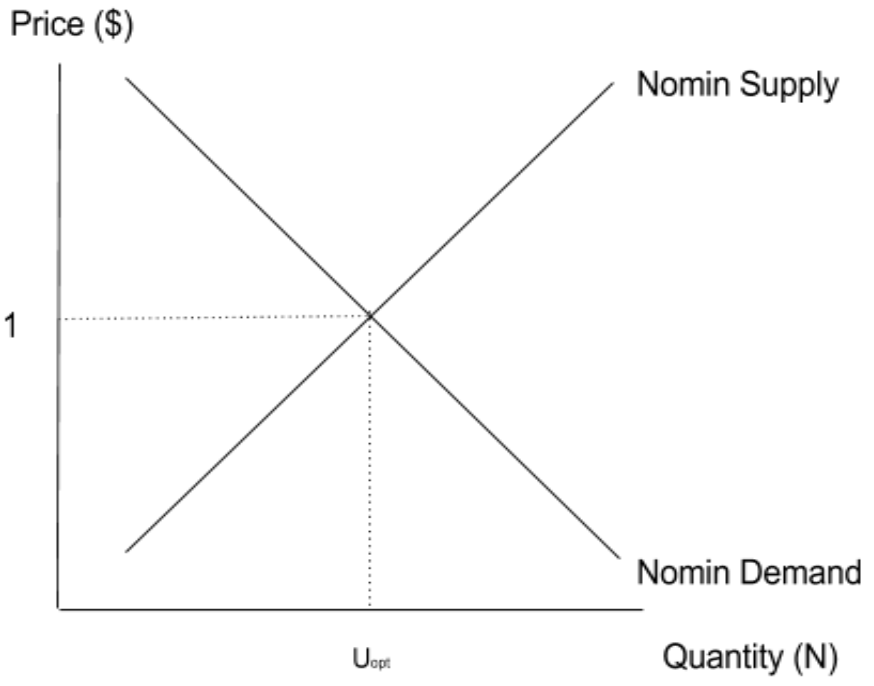
\includegraphics[width=.7\textwidth]{img/nomin-demand-vs-supply}
\end{figure}

\subsubsection*{Demand}

\noindent The system is unable to influence the demand for \NOM{}. It will come primarily from the utility of a stable Nomin.

\subsubsection*{Supply}

\noindent However, the supply of \NOM{} is controlled directly by the Havven holders, who use the system to issue and burn \NOM{}. This means the system can provide incentives for Havven holders to expand and contract the \NOM{} supply when demand changes. \\

\noindent The goal of Havven is to incentivise the Havven holders to maintain the level of \NOM{} supply at $U_{opt}$, such that $P_n = 1$. In order to do this, the system must provide incentives to the \HAV{} token holders.  \\

\newpage

\subsection{Transaction Fees} Every time a Nomin transaction occurs, the Havven system charges a small transaction fee. Transaction fees allow the system to generate revenue, which it can distribute to \HAV{} holders as an incentive to maintain \NOM{} supply at $U_{opt}$. \\

\begin{namedthm}{Fees Charged (per transaction)}[]
$$ a_c = k.$$
\end{namedthm}

\noindent The fee charged on Nomin transactions is constant and will be sufficiently small that it provides little to no friction for the user. \\

\begin{figure}[h!]
    \centering
    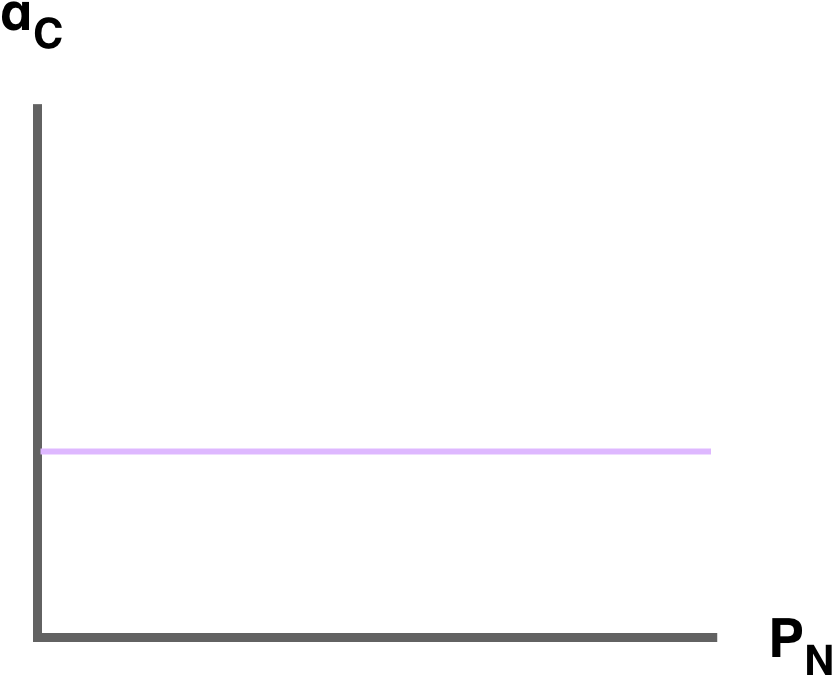
\includegraphics[width=.55\textwidth]{img/fees-charged}
\end{figure}

\newpage

\begin{namedthm}{Fees Received (per escrower)}[]
\[
\alpha_r = 
\begin{cases}
 \frac{\alpha_{base}}{U_{opt}} * U_I &\mbox{when } U_I \leq U_{opt}, \\ 
 \frac{\alpha_{base}}{U_{max} - U_{opt}} * (U_I  - U_{max}) &\mbox{when } U_{opt} \leq U_I \leq U_{max}, \\ 
 0 &\mbox{otherwise}.
 \end{cases}
\]
\end{namedthm}

\begin{figure}[h!]
    \centering
    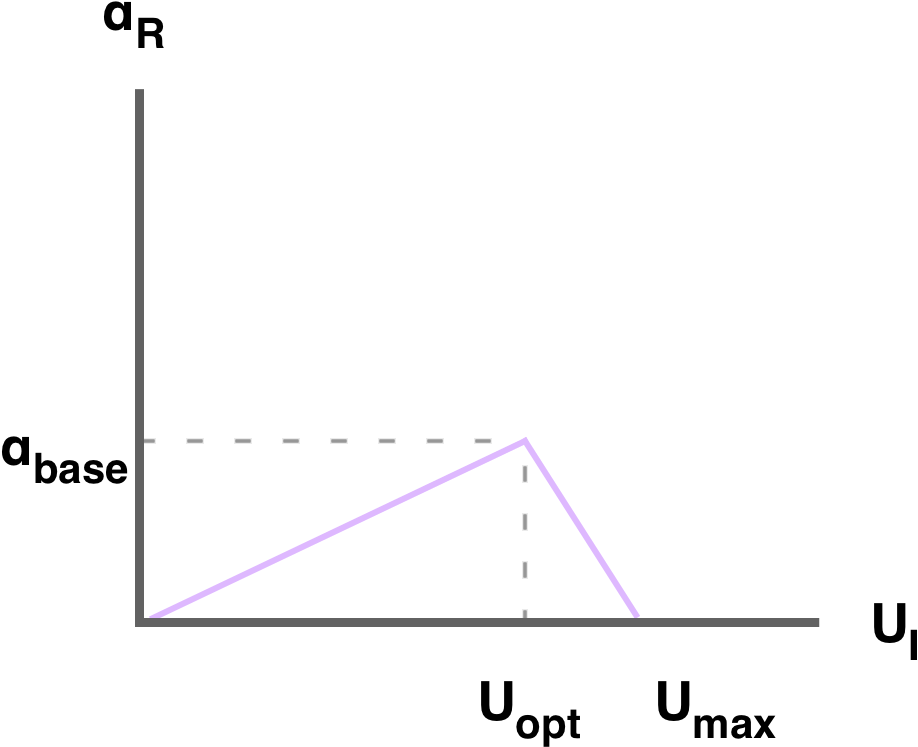
\includegraphics[width=.55\textwidth]{img/fees-received}
\end{figure}

\noindent Fees are only paid to \HAV{} holders who have elected to escrow, as a reward for collateralising the system. The fees received increases linearly to a maximum at the optimal utilisation ratio $U_{opt}$. However, the fees quickly diminish as $U_I$ approaches $U_{max}$ and drop to nothing after this point. \\

\noindent Intuitively, this equation encourages \HAV{} holders who have escrowed to maintain their $U_I$ at $U_{opt}$. 

\newpage

\noindent Recall the concept of the utilisation ratio, which was introduced earlier:

$$ U = \frac{P_n * N}{P_h * H}. $$ \\

\noindent We have introduced the concept of an optimal utilisation ratio and its importance in achieving Havven's  goal $P_n = 1$. Havven's fee structure encourages all \HAV{} holders who escrow to maintain their personal utilisation ratio $U_I$ at $U_{opt}$. However, the system needs a function to determine what $U_{opt}$ is. \\

\noindent If $P_n > 1$ then the system must encourage more \NOM{} to be issued. If $P_n < 1$ the system must encourage \NOM{} to be burned. The definition of $U_{opt}$ must provide this incentive. \\

\begin{namedthm}{Optimal Utilisation Ratio}[]
$$ U_{opt} = f(P_n) * U,$$
$$ f(x) = max(\sigma * (x - 1)^{\phi} + 1, 0), $$
$$\text{where } 0 \leq \sigma, \text{ the price sensitivity parameter}, $$
$$\phi \geq 1, \text{ the flattening parameter}. $$
\end{namedthm}

\begin{figure}[h!]
    \centering
    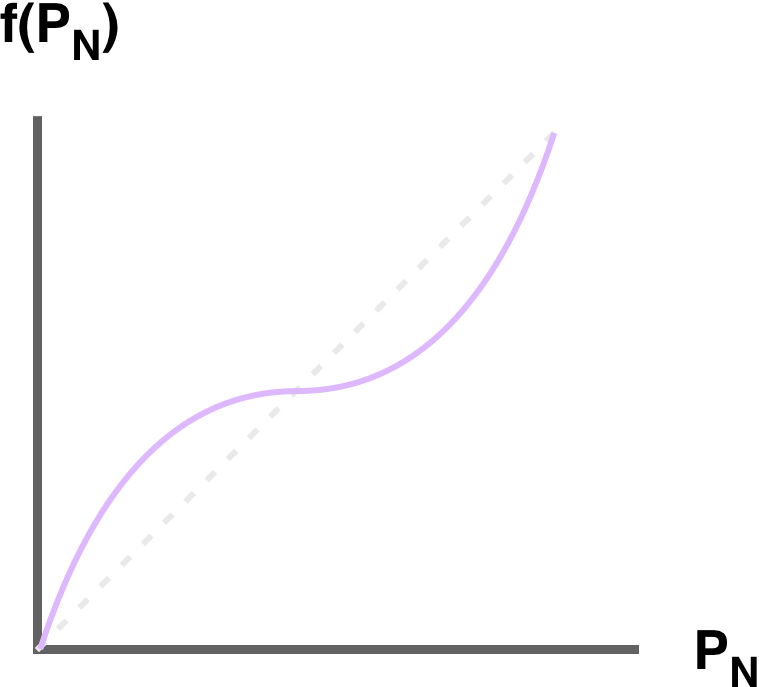
\includegraphics[width=.5\textwidth]{img/U_opt}
\end{figure}

\noindent The graph above shows that the when $P_n$ is near \$1, f'(x) is small. However, the further $P_n$ diverges from \$1, the larger the derivative becomes. This means the incentive to move toward $U_{opt}$ increases as $P_n$ diverges from \$1.

\newpage

\subsection*{Maximum Utilisation Ratio}

\noindent When we discussed the concept of issuing \NOM{}, we introduced the idea of a maximum utilisation ratio, $U_{max}$. Havven needs to maintain $U < U_{max} < 1$, in order to remain overcapitalised. It might seem intuitive that $U_{max}$ should be a static value. However, since $U_{opt}$ changes linearly with $P_n$ and inversely with $P_h$, there are several situations where $U_{max}$ may need to change. Below we define $U_{max}$.

\begin{namedthm}{}[]
\[
U_{max} = 
\begin{cases}
 U_{base} &\mbox{when } U_{opt} \leq U_{base}, \\ 
 \alpha * U_{opt} &\mbox{otherwise}.
 \end{cases}
\]
\end{namedthm}

\begin{figure}[h!]
    \centering
    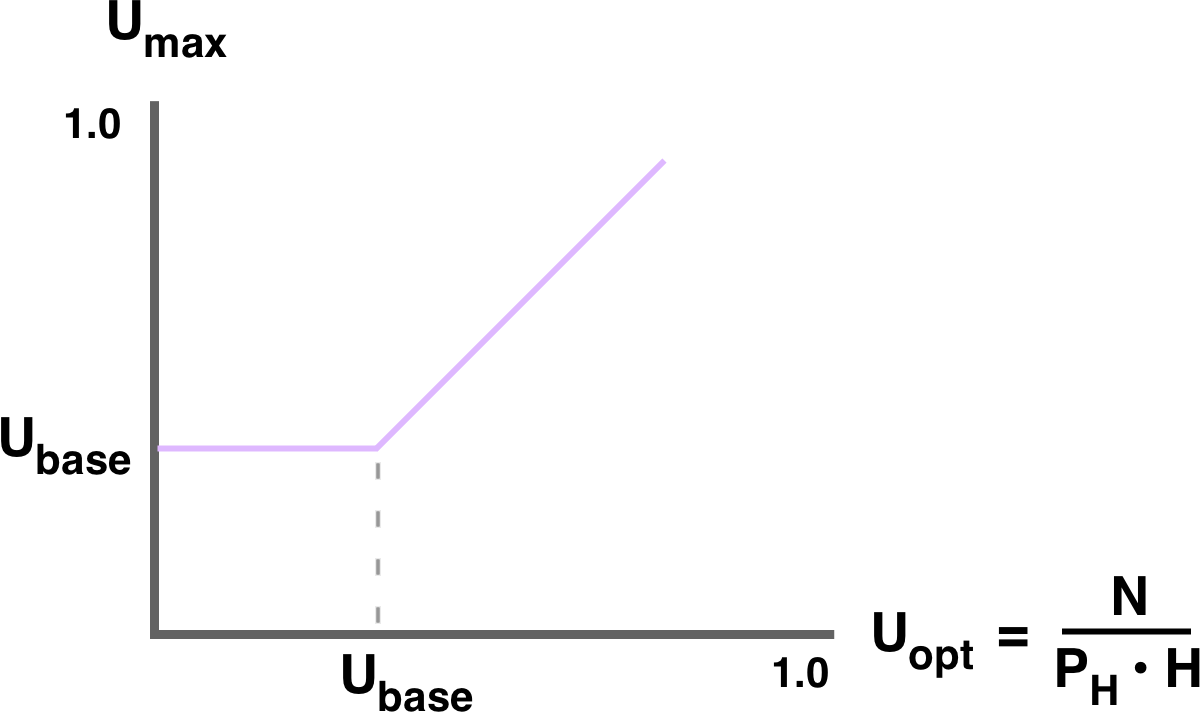
\includegraphics[width=.75\textwidth]{img/U_max}
\end{figure}

\newpage

\subsection{Intrinsic Havven Price} With the \HAV{} token being ERC20 compliant, it will have a market price on both decentralised and centralised exchanges. \\

\noindent While the system will access the market price via an oracle, it is also beneficial to define a $P_h$ that can be determined internally, thus avoiding the impact of speculation. Ignoring speculative demand, $P_h$ can be expressed as a function of the transaction fees that the system charges. Below we define an initial iteration of the intrinsic $P_h$.

\begin{namedthm}{Havven Price}[]
\begin{align*} 
P_{h,t} &= \frac{1}{H}* \sum\limits_{t=1}^\infty \frac{d_{n,t} *v_{n,t} * \alpha_{R,t}}{(1+R)^t} \approx \frac{d_{n,t} *v_{n,t} * \alpha_{R,t}}{R * H}, \\
& P_{h,t} \text{ is the price of one \HAV{} at time } t, \\
& H \text{ is the number of havvens}, \\
& d_{n,t} \text{ is the demand for \NOM{} at t}, \\
& v_{n,t} \text{ is the velocity of \NOM{} at t}, \\
& \alpha_{R,t} \text{ is the fee from trade with \NOM{}}, \\
& R \text{ is the interest rate / rate of return of havvens}. \\
\end{align*}
\end{namedthm}

\newpage

\subsection{Juans Description of Players (Refactored)}
\begin{namedthm}{Havven Holder}[]
An investor who owns \HAV{} tokens.
\end{namedthm}

\noindent In order to purchase \HAV{} the expected return has to be greater than that of alternative investments (opportunity cost). The expected return of \HAV{} comes from:
\begin{enumerate}
\item{The fees received on escrowed \HAV{}.}
\item{An increase in $P_h$.}
\item{Seigniorage (i.e., an increment in $P_h$ implies that the investor can issue more \NOM{}, which may eventually have a larger value than his original investment.}
\end{enumerate}

\noindent At any moment in time, the investor must decide:
\begin{enumerate}
\item{Whether or not to issue new \NOM{} (assuming $U_I < U_{max}$), or to burn some of them. All \NOM{} are issued/burnt at the prevailing market exchange rate, denominated in ETH.}
\item{Whether to sell some quantity of \HAV{} in the market at price $P^M_{h,t}$. Only \HAV{} which haven't been escrowed can be sold. Otherwise they must burn \NOM{} to release them. }
\end{enumerate}

\begin{namedthm}{Nomin User}[]
A person who uses the Nomin token.
\end{namedthm}
 
\noindent In order to purchase \NOM{}, it must provide the user more utility than USD, since both have the same consumption value in the market. This utility may come from the properties of crypto. \\

\noindent At any time, they must decide: 
\begin{enumerate}
\item{Whether to buy or to sell \NOM{} at $P_n$.}
\end{enumerate}

\newpage